\documentclass[a4paper]{article}

\usepackage[english]{babel}
\usepackage[utf8]{inputenc}
\usepackage{amsmath}
\usepackage[dvipsnames]{xcolor}
\usepackage{graphicx}
\usepackage[colorinlistoftodos]{todonotes}
\usepackage{listings}
\usepackage{enumitem}
\usetikzlibrary{fit}
\usetikzlibrary{calc}
\usepackage{mdframed}
\usepackage{cite}
\usepackage[margin=1in]{geometry}
\usepackage{floatrow}
\usepackage{fancyvrb}
\usepackage[margin=1cm]{caption}
\usepackage{titlesec}

\setcounter{secnumdepth}{4}


\titleformat{\paragraph}
{\normalfont\normalsize\bfseries}{\theparagraph}{1em}{}
\titlespacing*{\paragraph}
{0pt}{3.25ex plus 1ex minus .2ex}{1.5ex plus .2ex}
 

\newlist{inlinelist}{enumerate*}{1}
\setlist*[inlinelist,1]{%
  label=(\roman*),
}

% redefine \VerbatimInput
\RecustomVerbatimCommand{\VerbatimInput}{VerbatimInput}%
{fontsize=\footnotesize,
 %
 frame=lines,  % top and bottom rule only
 framesep=2em, % separation between frame and text
 rulecolor=\color{Gray},
 %
 label=\fbox{\color{Black}Results},
 labelposition=topline,
 %
 commandchars=\|\(\), % escape character and argument delimiters for
                      % commands within the verbatim
 commentchar=*        % comment character
}





\title{Body-Headline Latent Dirichilet Allocation}

\author{Prateek Gupta (UNI: pg2455)}

\date{\today}

\begin{document}
\maketitle

\begin{abstract}
Topic models have been successfully applied to various types of unstructured datasets. Specifically in the world of natural language processing these tools have found wide applications in uncovering hidden topic distributions in documents. The problem we have considered relates to uncovering hidden structure of a text article at much more granular level as compared to only the article body. We relate the topic distribution of article's headline to the topic distribution of its body. This method can be extended further to paragraph level making it easier to find the topic distributions at each level. We conduct experiments on \textit{The New York Times} corpus to find out \textit{how much the body speaks of its headline}. We also discuss the wide applicability of this model.
\end{abstract}

\section{Introduction}
Statistical topic models have been extensively applied to uncover the hidden insights from grouped data like text articles where each article is a collection of words. \emph{Latent Dirichlet Allocation (LDA)} model can help in arranging large unstructured collection of articles according to inferred topics from the model \cite{blei_prob_model_paper}. 

Traditionally topic models have been applied separately on body\cite{blei_prob_model_paper, lda_blei} and tweets\cite{tm_lda} which are short collection of words like headlines. Since headline is crafted in a manner such that it represents main theme of the body content we expect that topics represented in headline should be a subset of topics represented in body. In this work we develop the \emph{Body-Headline Latent Dirichlet Allocation} (BHLDA) model which captures such an influence of body topics on headline topics and vice versa. We expect to get body topics such that headline topics are subset of it. This \emph{subset property} can not be confirmed in \emph{normal LDA} on body and headline owing to the lack of correspondence between headline topics and body topics.

\emph{LDA} computes article topics from body content but it can be computationally expensive owing to the large number of words in body. The \emph{BHLDA} model can enable the user to compute document topics by using the words from headline, the vocabulary of which is small compared to that of the body, thus ensuring relatively cheap computations. Because of the way the model is designed, word distribution of body topics influences word distribution of headline topics and vice-versa. \emph{Headline Only LDA} can also perform cheap computations but headline topic distribution will be completely independent of body topic distribution. We expect results of topic inference from headline in BHLDA to be more appropriate as compared to \emph{Headline Only LDA}.

The idea of \emph{BHLDA} model extends beyond just the headline and the body. For example, it can be used to infer topics at article's abstract and paragraph level too. Thus, we think of \emph{BHLDA} as a special case of \emph{Microlevel LDA} which can involve applying LDA at various levels of an article. LDA at various levels is possible when there is a structure in grouped data. For example, images and their captions is an example of grouped data with structure \cite{model_annotated_data}. Thus, BHLDA model can also find its application in the domain out of text.

Although the idea of \emph{BHLDA} model was conceived independently of any work done yet, we looked at work that uses similar ideas of graphical models. Literature survey indicates that there have been similar graphical model but applied in entirely different context. 

Polylingual topic models \cite{ptm} is a way to find topics aligned across various language versions of the same article. Graphical model used in the paper is similar to the \emph{BHLDA} model. Structure in grouped data has lots of implication for modeling purposes. Research paper\cite{model_annotated_data} considers this problem in depth and proposed various models along with their upside as well as downsides. Paper discusses various models for correlating topics in images through their pixel level information and image captions.

In this paper we discuss the \emph{BHLDA} model and derive its inference procedure used for parameter estimation. We discuss results using The New York Times Corpus \cite{corpus}.  We compare its performance with \emph{Body Only LDA} and \emph{Headline Only LDA}. We wind up by pointing to future work needed to verify the results even more concretely and discuss few applications that this model can promise. We find that \emph{BHLDA} model gives direct correspondence between word distribution in headline topics and body topics which otherwise is not possible in \emph{Headline Only LDA} and \emph{Body Only LDA}. Also the word distribution of headline and body topics are more similar in \emph{BHLDA} model as compared to \emph{normal LDA} on headline and body. In order to enable the reader with access to the code to enable self-experiments we have shifted our work on Github repo 'vewpoint' of 'prateekpg2455'.

\section{BHLDA Model}

\subsection{Notations}
Variables in bold letters denote matrix.
\emph{N} is number of words in a document. $\hat{N}$ is number of words in headline. \emph{D} is number of documents in the corpus. \emph{V} is number of words in vocabulary. \emph{K} is number of topics. $\mathbf{W} = [w_{j,t}]_{j=1, t=1}^{D, N}$ represents body word matrix where $w_{j,t}$ is the $t^{th}$ body word in $j^{th}$ document. $\mathbf{\hat{W}} = [w_{j,\hat{t}}]_{j=1,\hat{t}=1}^{D,\hat{N}}$ where $w_{j,\hat{t}}$ is the $\hat{t}^{th}$ headline word in $j^{th}$ document. $\mathbf{Z} = [z_{j,t}]_{j=1, t=1}^{D, N}$ represents matrix of topic allocation to words in the body where $z_{j,t}$ is topic allocation to $t^{th}$ body word in $j^{th}$ document. It is of same dimension as $\mathbf{W}$. Similar description holds for  $\mathbf{\hat{Z}} = [z_{j,\hat{t}}]_{j=1, \hat{t}=1}^{D, \hat{N}}$. $\mathbf{\Theta} = [\theta_{j,i}]_{j=1,i=1}^{D,N}$ represents $i^{th}$ topic proportion of $j^{th}$ document/article. $\theta_{j}$ represents topic distribution vector for a document. $\mathbf{\Psi} =  [\psi_{i,r}]_{i=1, r=1}^{K,V}$ where $\psi_{i,r}$ is probability of choosing $r^{th}$ word for body from $i^{th}$ body topic. $\psi_{i}$ is the multinomial distribution vector for $i^{th}$ topic. $\mathbf{\hat{\Psi}} =  [\hat{\psi}_{i,r}]_{i=1, r=1}^{K,V}$ where $\hat{\psi}_{i,r}$ is probability of choosing $r^{th}$ word for headline from $i^{th}$ headline topic. 
Detailed description of variables, their size and representation in the model is given in Appendix \ref{notations}.

\subsection{Generative Model}
Topic distribution for document $\textit{j}$ is generated from Dirichlet distribution with parameter \textit{$\alpha$}. Given the topic distribution \textit{$\theta_{j}$}, \textit{N} topic allocations for body are sampled from multinomial distribution with parameter \textit{$\theta_{j}$}. Similarly, \textit{$\hat{N}$} topic allocations are sampled for headline. For each topic allocation sampled, a word is generated from that topic. Thus, this model captures the fact that topic allocations for body and headline can differ because of large number of words in the body as compared to the headline. 

The \textit{Body-Headline LDA} (BHLDA) model, shown in Figure \ref{fig: model} assumes following generative process:
\begin{enumerate}
\item Sample K Dirichlet random variables for body topic distribution, $\psi_{i} \sim \textit{Dir($\beta$)}$
\item Sample K Dirichilet random variables for headline topic distribution, $\hat{\psi}_{i} \sim \textit{Dir($\hat{\beta}$)}$ 
\item For each document j, sample a Dirichlet random variable, $\theta_{j} \sim \textit{Dir($\alpha$)}$
\begin{enumerate}[label =(\alph*)]
\item For each word $w_{j,t}$ in body
\begin{enumerate}
\item Sample a body topic, $z_{j,t} \sim \textit{Mult($\theta_{j}$)}$
\item Sample a body word, $w_{j,t} \sim \textit{Mult($\psi_{z}$)}$
\end{enumerate}
\item For each word $\hat{w}_{j,\hat{t}}$ in headline
\begin{enumerate}
\item Sample a headline topic, $\hat{z}_{j,\hat{t}} \sim \textit{Mult($\theta_{j}$)}$
\item Sample a headline word, $\hat{w}_{j,\hat{t}} \sim \textit{Mult($\hat{\psi}_{\hat{z}}$)}$
\end{enumerate} 
\end{enumerate}
\end{enumerate}

\subsection{Graphical Model}
Model specifying the relation between variables is shown in Figure \ref{fig: model}. Graphical model assumes that topic allocations $\hat{z}$  in headline and $z$ in body  influence each other through topic distribution $\theta$. Sampling of words in body and headline are dependent on topic distribution $\theta_{j}$. Thus topic allocations in the body are influenced by topic allocations in the headline and vice versa.

Topic distribution over one article does not depend on topic distribution of other documents implying exchangeability within $\theta_{j}$ vectors. Similarly, words within body are exchangeable and so are words within headline. 

V-structure formed at $\psi$ and $\hat{\psi}$ assures that influence from topic allocations flows from $z$ or $\hat{z}$ to $\psi$ and $\hat{\psi}$. Since there is an influence from $z$ to $\hat{z}$, $\psi$ and $\hat{\psi}$ influences each other which generates correspondence between headline topics and body topics. 

\begin{figure}  \label{model}
\centering
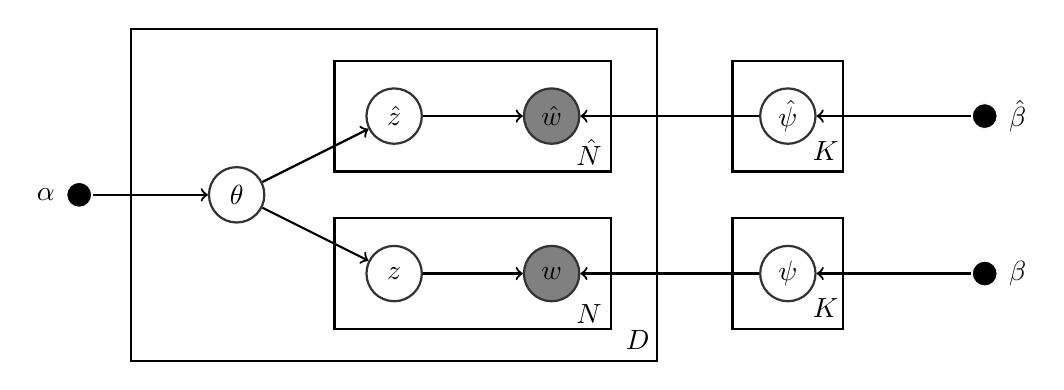
\begin{tikzpicture}[thick]
\tikzstyle{priors}=[circle,minimum size =1, thick, draw=black!2, node distance = 10mm, fill =black]
\tikzstyle{main}=[circle, minimum size = 20, thick, draw =black!80, node distance = 16mm, fill= white]

	%circles
	\node[priors] (prior) at (0,1) [label=left:$\alpha$] { };
	\node[main] (theta) at (2,1) [label = center:$\theta$] { };
	\node[main] (z)  at (4,0) [label = center:$z$] { } ;
	\node[main] (w) at (6,0) [label = center:$w$, fill = gray] {};
	\node[main] (psi) at (9,0) [label = center:$\psi$] { };
	\node[priors] (beta) at (11.5,0) [label = right:$\beta$]{};
	\node[main] (z_hat)  at (4,2) [label =  center:$\hat{z}$]{};
	\node[main] (w_hat) at (6,2) [label =  center:$\hat{w}$, fill = gray]{};
	\node[main] (psi_hat) at (9,2) [label=center:$\hat{\psi}$] {};
	\node[priors] (beta_hat) at (11.5,2) [label = right:$\hat{\beta}$]{};
	%paths
	\draw[->] (prior) -- (theta) ;
	\draw[->] (theta) -- (z);
	\draw[->] (theta) -- (z_hat);
	\draw[->] (z) -- (w);
	\draw[->] (z_hat) -- (w_hat);
	\draw[->] (psi) -- (w);
	\draw[->] (psi_hat) -- (w_hat);
	\draw[->] (beta) -- (psi);
	\draw[->] (beta_hat) -- (psi_hat);
	
	%rectangles
	\node[draw, minimum height = 12em, minimum width = 19em,fit=(theta) (z)(w) (z_hat)(w_hat)]  (doc_plate) [label={[xshift=8.8em, yshift=-12em]$D$}]{};
	\node[draw, minimum height = 4em, minimum width = 10em, fit =(z)(w)] (body_plate) [label={[xshift=4.2em, yshift=-4.2em]$N$}] { };
	\node[draw, minimum height = 4em, minimum width = 10em, fit =(z_hat)(w_hat)] (head_plate) [label={[xshift=4.2em, yshift=-4.2em]$\hat{N}$}] { };
	\node[draw,minimum height = 4em, minimum width = 4em, fit = (psi)] (body_K) [label = {[label distance = -0.75cm]south east:$K$}]{};
	\node[draw, minimum height = 4em, minimum width =4em, fit = (psi_hat)] (head_K) [label = {[label distance  = -0.75cm]south east:$K$}]{};
	

\end{tikzpicture}
\caption{BHLDA Graphical Model} \label{fig: model}
\end{figure}

\subsection{Joint Distribution}
The resulting joint distribution on body words, headline words and latent variables is given by 

\begin{multline}
P(\mathbf{\Psi}, \mathbf{\hat{\Psi}}, \mathbf{\Theta},  \mathbf{Z}, \mathbf{\hat{Z}}, \mathbf{W}, \mathbf{\hat{W}} ; \alpha, \beta) =  \\
\prod_{i=1}^{K} P(\psi_{i} \mid \beta) \prod_{i=1}^{K} P(\hat{\psi}_{i} \mid \hat{\beta}) \prod_{j=1}^{D} P(\theta_{j} \mid \alpha) \prod_{t=1}^{N} P(z_{j,t} \mid \theta_{j})P(w_{j,t} \mid \psi_{z_{j,t}}) \prod_{\hat{t}=1}^{\hat{N}} P(\hat{z}_{j,t} \mid \theta_{j})P(\hat{w}_{j,t} \mid \hat{\psi}_{\hat{z}_{j,t}})
\end{multline}

Reader is advised to refer Appendix \ref{derivation} for detailed derivation of above equation.
\section{Inference and Estimation}

Collapsed Gibbs Sampling for the model is derived in Appendix \ref{derivation}. Update equations derived are as follows:
\begin{enumerate}
\item For body words,
  \begin{displaymath}
   P(z_{m,n} = k \mid \mathbf{W}, \mathbf{\hat{W}}, \mathbf{Z_{-(m,n)}}, \mathbf{\hat{Z}} ; \alpha, \beta ) 
 \propto \\ 
 \left( \alpha_{k} + n_{m,(.)}^{k,-(m,n)} + \hat{n}_{m,(.)}^{k} \right) \times \left( \frac{\beta_{\nu} + n_{(.),\nu}^{k,-(m,n)}}{\sum_{r=1}^{V}(\beta_{r} + n_{(.),r}^{k,-(m,n)})} \right)
  \end{displaymath} 
  
\item For headline words,
  \begin{displaymath}
   P(\hat{z}_{m,n} = k \mid \mathbf{W}, \mathbf{\hat{W}}, \mathbf{Z}, \mathbf{\hat{Z}_{-(m,n)}} ; \alpha, \beta ) 
 \propto \\ 
 \left( \alpha_{k} + n_{m,(.)}^{k} + \hat{n}_{m,(.)}^{k,-(m,n)} \right) \times \left( \frac{\hat{\beta}_{\nu} + \hat{n}_{(.),\nu}^{k,-(m,n)}}{\sum_{r=1}^{V}(\hat{\beta}_{r} + \hat{n}_{(.),r}^{k,-(m,n)})} \right)
  \end{displaymath}
\end{enumerate}

Above equations implies that conditional distribution of $n^{th}$ word in the $m^{th}$ document belonging to $k^{th}$ topic is directly proportional to $\alpha_{k}$ and number of words other than $w_{m,n}$ that belong to $k^{th}$ topic in $m^{th}$ document and it befits intuition. Interestingly enough, conditional probability of $z_{m,n}=k$ is also influenced by number of headline words belonging to $k^{th}$ topic. Thus, model supports the relation between headline topics and body topics as expected. Assuming $w_{m,n} = \nu$, conditional probability of $z_{m,n}=k$ is proportional to number of times $\nu$ has been allocated to $k^{th}$ topic across the corpus except $w_{m,n}$. Similar conclusions can be drawn for conditional probability of  $\hat{z}_{m,n} = k$. 

Conditional probability of $z_{m,n} = k$ is in terms of present state of topic allocations except the $z_{m,n}^{th}$ term which is atypical of Gibbs Sampling method. 


\section{Data}
We used \textit{The New York Times Annotated Corpus} \cite{corpus} to test our model. The corpus contains 1.8 million articles. Each article is a collection of article text and related metadata like author name, editor name, publication date, online section of published article, newspaper section as well as page number and column number of published article, manually annotated tags, headline and much more. Each article is referred to by its unique id. Detailed process of preprocessing steps and issues dealt with such a huge corpus are discussed in Appendix \ref{data}

\section{Results}
The $BHLDA$ model was run on 100,000 articles of \emph{The New York Times Corpus}. Numbers of articles were chosen such that the model can handle computations of Gibbs Sampling procedure. Appendix \ref{BHLDA output} shows the results of BHLDA model. Appendix \ref{body lda output} and \ref{headline lda output} displays output of \emph{Body Only LDA} and \emph{Headline Only LDA}. 

One direct advantage of \emph{BHLDA} model is that the output word distribution for each topic has one to one correspondence between body and headline. This is not possible in case of normal LDA run on only body or only headline. This result is shown in Figure \ref{fig: snippet}. 

\begin{figure}[ht]
		\begin{center}
		% Include the eps file, scale it such that it's width equals the column width. You can also put width=8cm for example...
		\includegraphics[width=\columnwidth]{snippet.jpeg}
		\caption{Snippet of Results}
		\label{fig: snippet}
		\end{center}
\end{figure}

Uniqueness of topics in \emph{BHLDA} is evident from the Table \ref{tab: KL}. For each topic, there exists unique topic in \emph{BHLDA} while there are potential matches in \emph{Body Only LDA} and \emph{Headline Only LDA}. It is also evident from the results in section \ref{word_bhlda}, \ref{body lda output}, \ref{headline lda output}  by manually reading words in word distributions. 

A sample of final topic allocations to articles is shown in Appendix \ref{topics_bhlda}. Topic allocations to headline words are sparse as compared to topic allocations to body words. It follows from intuition because of the presence of relatively fewer headline words as compared to the body words. Topic allocations in \emph{Headline Only LDA} are also sparse but are completely independent of body words. 
As far as the sparsity is concerned headline topic distribution in \emph{BHLDA} is not as sparse as in \emph{Headline Only LDA}. As an evidence, across 100,000 articles, there were 91,268 articles in which number of non-zero entries in headline topic distribution for \emph{BHLDA} was more than that for \emph{Headline Only LDA}. This means \emph{BHLDA} does loose on sparsity for  headline topic distributions.

\emph{Kulback-Leibler Divergence} of two multinomial distribution is defined as 
$KL(p||q) = \sum_{i=1} p_{i} \times ln(\frac{p_{i}}{q_{i}})$, where terms with $p_{i} = 0$ are simply put as 0 because $\lim_{x\to 0}x \times ln(x) = 0$. Please note that KL Divergence considers only the support of $q$ for its computation. Only few topics from normal LDA on body and headline were found to be similar. For example, correspondence between body LDA and headline LDA can be drawn through topic 0 and topic 5 respectively.  Similar topic can be found in BHLDA model at topic 14. Table \ref{tab: KL} displays such pairs of topics and corresponding KL Divergence for both the models. 

It is interesting to note that word distribution for body topics and headline topics in \emph{BHLDA} are more closer i.e. they have lower average KL Divergence as compared to \emph{normal LDA} on body and headline only. At the same time, uniqueness of topics in \emph{BHLDA} can also be confirmed from the Table \ref{tab: KL}.

\begin{table}[htbp]
\centering
\caption{KL Divergence between word distributions for LDA and BHLDA. p is topic number in \emph{Body only LDA} and q is corresponding topic number in \emph{Headline only LDA}. z is corresponding topic number in \emph{BHLDA}. $body_{*}$ and $headline_{*}$ are word distribution of topics. Matching of topics in LDA is subjective. Average includes minimum values in each observation. Negative values of KL Divergence are because of inadequate storage of float values. Note that there can be multiple matches for each Topic. They are separated by '/'.}

\begin{tabular}{c | c c | c c}
\hline \hline
 & \multicolumn{2}{c}{LDA} & \multicolumn{2}{c}{BHLDA} \\
\hline
 Topic & \emph{p,q} & $KL(body_{p}||headline_{q})$ & \emph{z} & $KL(body_{z} || headline_{z})$ \\
\hline
National Budget & 0,5 & 0.3599 & 14 & 0.1827 \\
International Affairs & 13,7 & 0.2749 & 7 & 0.2109 \\
Dance/Theater/Music & 14,0/14,6 & 0.2692/0.3037 & 6 & 0.0280 \\
Art/Music/Travel & 19,0/19,6 & 0.0598/0.0856 & 0 & -0.0143 \\
Markets/Finance & 18,1/18,2/18,12 & 0.1498/0.3177/-0.0372 & 4/9 & 0.3614/0.4187\\
Sports & 17,11/16,11 & 0.3976/0.3354 & 5/15 & 0.1963/0.2360\\
\hline
& Average & 0.2103 & & 0.1608\\
\hline
\end{tabular}
\label{tab: KL}
\end{table}

Majority of headline topics were found to be a subset of body topics. Results indicate that there were 2,658 articles in which headline topics were not subset of body topics. Thus, 97.342\% times headline topics were subset of body topics. 

\section{Future Work}
Present results were obtained using uniform priors on $\beta$ and $\alpha$. More informative priors can improve the results drastically. As per the figure \ref{fig: priors}, it is quite evident that word distribution for headline and body differ a lot. As per the plot \ref{fig: priors}, cumulative distribution function differ a lot for body words and headline words. Thus, $\beta$ and $\hat{\beta}$ should be initialized differently for better results. 

Problem of aligning word distribution of \emph{Body Only LDA} with \emph{Headline Only LDA} can be addressed by seeding \emph{Headline Only LDA} with the results from \emph{Body Only LDA}. Thus, results on KL Divergence can be verified even further after running LDA this way. 

Running BHLDA based on \emph{stochastic variational inference} can speed up the computations and hence can be used to verify the results based on even larger number of articles. Present work uses Collapsed Gibbs Sampling method for inference and estimation and hence we cannot scale up the model to larger number of articles. 

Generation of headline words just from body words and body words just from headline words can be another useful metric to compare normal LDA and BHLDA. Thus, mathematical formulation to compute maximum likelihood estimates of conditional distribution can aid in performing this analysis. Metrics like perplexity and posterior predictive checks can also help in verifying the results of \emph{BHLDA} model. 

\section{BHLDA: Applications and extension} \label{application}
News article recommendation is a common problem in many news organizations that helps them in keeping the reader engaged to their websites. It is a common behavior of any reader to infer topics from the headline and then decide whether to read an article or not. Thus, ability to infer topics at various levels of the text article which is facilitated by \emph{BHLDA} model can be useful in recommendation engines. For example, a recommendation engine with features as topics inferred from headline text can take into account reading behavior of readers. As discussed, headline topics inferred in this manner are more appropriate as compared to \emph{Headline Only LDA} which can enable the recommendation engine to incorporate features from headline topics that reflect body topics more closely. Thus, although recommendation engine includes features only from headline it is able to incorporate body features too and hence recommendation is influenced by body and headline topics using computations involving only the headline words. 

Summarizing an article is the problem that deals with identifying main theme in the article and displaying that as description of the article. Some news organization just displays first 3 sentences of the article along with headlines to give the flavor of an article. An article contains multiple paragraphs. Each paragraph represents different topic distribution. \emph{Microlevel LDA} can help in this problem. LDA at each level of article i.e. paragraphs can give topic allocations of all the paragraphs. Assuming that paragraph with topic allocations similar to headline topic allocations are more reflective of headline content is true, summary of article can be given by paragraph with similar topic distribution as that of headline.

It enable cheaper computation of article topics using only the headline words. Owing to the fewer number of headline words as compared to body words, computation of topics from headline words is relatively cheaper as compared to that from body words and \emph{BHLDA} model enables appropriate representation of topics influenced also by the body words.

%Uncovering intentions behind search queries in search engine: Many times a search query on search engine can imply various intentions of the user. For example, a search query 'Google Nexus 5' can have various intentions like:\begin{inlinelist}\item Specifications of Nexus 5 \item Deals on Nexus 5 \item Places to buy Nexus 5 \item Recent news related to Nexus 5 \end{inlinelist}. Using search queries as headline and content of article clicked as body will give different topic allocations for search string. Thus it can help in distinguishing between intentions. 
%


The \emph{BHLDA} model can be useful in establishing credibility of news publications. Some news sources have headlines crafted in a manner to attract more readers and does not reflect properly the contents of an article. Average KL Divergence of news sources can be used as a metric to quantify quality of news sources. 


\section{Appendix}

\subsection{Notations} \label{notations}
\subsubsection{Observed Data}
As discussed in Appendix \ref{data} words are represented by unique numbers for modeling purpose. Thus observed data, for purpose of our modeling, is represented by vector \textbf{W} for body and $\mathbf{\hat{W}}$ for headline. 

\[
\mathbf{W} = 
   	\begin{bmatrix}
    w_{11} & w_{12} & ... w_{1N}\\	w_{21} & w_{22} & ... w_{2N}\\ ...\\ ...\\ ...\\  w_{D1} & w_{D2} & ... w_{DN}\\ \end{bmatrix} \quad
\mathbf{\hat{W}} = 
   	\begin{bmatrix}
    \hat{w}_{11} & \hat{w}_{12} & ... \hat{w}_{1\hat{N}}\\	\hat{w}_{21} & \hat{w}_{22} & ... \hat{w}_{2\hat{N}}\\ ...\\ ...\\ ...\\  \hat{w}_{D1} & \hat{w}_{D2} & ... \hat{w}_{D\hat{N}}\\ \end{bmatrix}
\]

where $w_{jt}, \hat{w}_{j\hat{t}} \in \{1,2,3 ... V \}$, V denotes number of words in vocabulary, N denotes number of words in document and $\hat{N}$ denotes number of words in headline.

\subsubsection{Latent Variables}

Figure \ref{fig: model} consists of various latent variables in the model. These variables are represented in a certain way for the purpose of our model representation. This section gives the view into how are the variables represented for the purpose of our code. 

Latent $Z$ variable represents association of words to a topic. It has same dimensions as of \textit{W} but the values taken by its elements are one of the \textit{K} topics. 

\[
\textbf{Z} = 
   	\begin{bmatrix}
    z_{11} & z_{12} & ... z_{1N}\\	z_{21} & z_{22} & ... z_{2N}\\ ...\\ ...\\ ...\\  z_{D1} & z_{D2} & ... z_{DN}\\ \end{bmatrix} \quad
\mathbf{\hat{Z}} = 
   	\begin{bmatrix}
    \hat{z}_{11} & \hat{z}_{12} & ... \hat{z}_{1\hat{N}}\\	\hat{z}_{21} & \hat{z}_{22} & ... \hat{z}_{2\hat{N}}\\ ...\\ ...\\ ...\\  \hat{z}_{D1} & \hat{z}_{D2} & ... \hat{z}_{D\hat{N}}\\ \end{bmatrix}
\]

where $z_{jt}, \hat{z}_{j\hat{t}} \in \{1,2,3 ... K \}$, K denotes number of topics and is specified by the user.

Topic distribution of each document$\theta$ is the hidden structure and represents the multinomial probability associated with the document. It can be interpreted as proportion of document representing $i^{th}$ topic.

\[
\mathbf{\Theta} = 
   	\begin{bmatrix}
    \theta_{11} & \theta_{12} & ... \theta_{1K}\\	\theta_{21} & \theta_{22} & ... \theta_{2K}\\ ...\\ ...\\ ...\\  \theta_{D1} & \theta_{D2} & ... \theta_{DK}\\ \end{bmatrix}
\]

where $\theta_{ij} \in [0,1], \sum_{j=1}^{K} \theta_{ij} = 1 $, K denotes number of topics and is specified by the user.

Probability distribution over words $\psi_{i}$ for each topic represents likelihood of word associated to that topic.

\[
\mathbf{\Psi} = 
   	\begin{bmatrix}
    \psi_{11} & \psi_{12} & ... \psi_{1V}\\	\psi_{21} & \psi_{22} & ... \psi_{2V}\\ ...\\ ...\\ ...\\  \psi_{K1} & \psi_{K2} & ... \psi_{KV}\\ \end{bmatrix} \quad
\mathbf{\hat{\Psi}} = 
   	\begin{bmatrix}
    \hat{\psi}_{11} & \hat{\psi}_{12} & ... \hat{\psi}_{1V}\\	\hat{\psi}_{21} & \hat{\psi}_{22} & ... \hat{\psi}_{2V}\\ ...\\ ...\\ ...\\  \hat{\psi}_{D1} & \hat{\psi}_{D2} & ... \hat{\psi}_{DV}\\ \end{bmatrix}
\]

where $\psi_{ir}, \hat{\psi}_{ir} \in [0,1], \sum_{r=1}^{V} \psi_{ir} = 1, \sum_{r=1}^{V} \hat{\psi}_{ir} = 1  $, V denotes number of words in vocabulary.

Priors in the model are represented by $\alpha$, $\beta$ and $\hat{\beta}$. Each of these latent variables are represented by vectors. 
\[
\mathbf{\alpha} = \begin{bmatrix} \alpha_{1} & \alpha_{2} & ... & \alpha_{K} \end{bmatrix}
\]
\[
\mathbf{\beta} = \begin{bmatrix} \beta_{1} & \beta_{2} & ... & \beta_{V} \end{bmatrix}
\]
\[
\mathbf{\hat{\beta}} = \begin{bmatrix} \hat{\beta}_{1} & \hat{\beta}_{2} & ... & \hat{\beta}_{V} \end{bmatrix}
\]


\subsection{Model Derivation} \label{derivation}

Throughout the derivation following notations are used:
\begin{itemize}
\setlength{\itemsep}{0.5pt}
\item i for $i^{th}$ topic, $i \in \{1,2,3 ... K\}$
\item j for $j^{th}$ document, $j \in \{1,2,3 ... D\}$
\item r for $r^{th}$ word in vocabulary, $r \in \{1,2,3 ... V\}$
\item t for $t^{th}$ word in a document, $t \in \{1,2,3 ... N\}$
\end{itemize}

Graphical model in Figure \ref{fig: model} suggests following joint distribution,
\begin{displaymath}
P(\mathbf{\Psi}, \mathbf{\hat{\Psi}}, \mathbf{\Theta},  \mathbf{Z}, \mathbf{\hat{Z}}, \mathbf{W}, \mathbf{\hat{W}} ; \alpha, \beta) = \\
P(\mathbf{\Psi} \mid \beta) P(\mathbf{\hat{\Psi}} \mid \hat{\beta}) P(\mathbf{\Theta} \mid \alpha) P(\mathbf{Z} \mid \mathbf{\Theta})P(\mathbf{W} \mid \mathbf{Z}) P(\mathbf{\hat{Z}} \mid \mathbf{\hat{\Theta}}) P(\mathbf{\hat{W}} \mid \mathbf{\hat{Z}})
\end{displaymath}

Following the independence assumptions implicit in the graphical model,
\begin{align*}
\begin{split}
P(\mathbf{\Psi}, \mathbf{\hat{\Psi}}, \mathbf{\Theta},  \mathbf{Z}, \mathbf{\hat{Z}}, \mathbf{W}, \mathbf{\hat{W}} ; \alpha, \beta)& = 
\prod_{i=1}^{K} P(\psi_{i} \mid \beta) \times \prod_{i=1}^{K} P(\hat{\psi}_{i} \mid \hat{\beta}) \times \prod_{j=1}^{D} P(\theta_{j} \mid \alpha) \times \prod_{t=1}^{N} P(z_{j,t} \mid \theta_{j})P(w_{j,t} \mid \psi_{z_{j,t}}) \\ 
& \quad \times \prod_{\hat{t}=1}^{\hat{N}} P(\hat{z}_{j,t} \mid \theta_{j})P(\hat{w}_{j,t} \mid \hat{\psi}_{\hat{z}_{j,t}})
\end{split}
\end{align*}

For the purpose of Gibbs sampling required distribution of words and associated topics which is given by, 
\begin{align*}
\begin{split}
P(\mathbf{Z}, \mathbf{\hat{Z}}, \mathbf{W}, \mathbf{\hat{W}} ; \alpha, \beta) &=  
\int_{\mathbf{\Theta}} \int_{\mathbf{\Psi}} \int_{\mathbf{\hat{\Psi}}} \prod_{i=1}^{K} P(\psi_{i} \mid \beta) \prod_{i=1}^{K} P(\hat{\psi}_{i} \mid \hat{\beta}) \prod_{j=1}^{D} P(\theta_{j} \mid \alpha) \prod_{t=1}^{N} P(z_{j,t} \mid \theta_{j})P(w_{j,t} \mid \psi_{z_{j,t}})\\
 & \quad \lefteqn{ \times \quad \prod_{\hat{t}=1}^{\hat{N}} P(\hat{z}_{j,t} \mid \theta_{j})P(\hat{w}_{j,t} \mid \hat{\psi}_{\hat{z}_{j,t}})\,d\mathbf{\Theta} \,d\mathbf{\Psi} \,d\mathbf{\hat{\Psi}}} \\
\end{split}
\end{align*}

\begin{multline*}
= \int_{\mathbf{\Psi}} \prod_{i=1}^{K} P(\psi_{i} \mid \beta) \prod_{j=1}^{D} \prod_{t=1}^{N}P(w_{j,t} \mid \psi_{z_{j,t}})\,d\mathbf{\Psi} \int_{\mathbf{\hat{\Psi}}} \prod_{i=1}^{K}P(\hat{\psi}_{i} \mid \hat{\beta}) \prod_{j=1}^{D} \prod_{\hat{t} =1}^{\hat{N}}P(\hat{w}_{j,\hat{t}} \mid \hat{\psi}_{\hat{z}_{j,\hat{t}}}) \,d\mathbf{\hat{\Psi}}
\\
\int_{\mathbf{\Theta}} \prod_{j=1}^{D}P(\theta_{j} \mid \alpha) \prod_{t=1}^{N} P(Z_{j,t} \mid \theta_{j})\prod_{\hat{t}=1}^{\hat{N}} P(\hat{z}_{j,\hat{t}} \mid \theta_{j})\,d\mathbf{\Theta}
\end{multline*}

Using the argument of exchangeability we can move product outside integration. 

\begin{multline*}
=\prod_{i=1}^{K}  \int_{\psi_{i}} P(\psi_{i} \mid \beta) \prod_{j=1}^{D} \prod_{t=1}^{N}P(w_{j,t} \mid \psi_{z_{j,t}})\,d\psi_{i} \times
\prod_{i=1}^{K} \int_{\hat{\psi}_{i}} P(\hat{\psi}_{i} \mid \hat{\beta}) \prod_{j=1}^{D} \prod_{\hat{t} =1}^{\hat{N}}P(\hat{w}_{j,\hat{t}} \mid \hat{\psi}_{\hat{z}_{j,\hat{t}}}) \,d\hat{\psi}_{i}\\
\times \prod_{j=1}^{D} \int_{\theta_{j}} P(\theta_{j} \mid \alpha) \prod_{t=1}^{N} P(Z_{j,t} \mid \theta_{j})\prod_{\hat{t}=1}^{\hat{N}} P(\hat{z}_{j,\hat{t}} \mid \theta_{j})\,d\mathbf{\theta_{\textit{j}}}
\end{multline*}

Following step relies on the fact that Dirichlet distribution is \textit{conjugate prior} to multinomial distribution. Also it uses the fact that integral of Dirichlet distribution is 1.
\begin{align*}
\begin{split}
\int_{\psi_{i}} P(\psi_{i} \mid \beta) \prod_{j=1}^{D} \prod_{t=1}^{N} P(w_{j,t} \mid \psi_{z_{j,t}}) \,d\psi_{i}
 = \int_{\psi_{i}} \frac{\Gamma(\sum_{r=1}^{V} \beta_{r})}{\prod_{r=1}^{V}\Gamma(\beta_{r})} \prod_{r=1}^{V} (\psi_{i,r})^{\beta_{r} -1} \prod_{r=1}^{V} (\psi_{i,r})^{n_{(.),r}^{i}}\,d\psi_{i}\\
  = \int_{\psi_{i}} \frac{\Gamma(\sum_{r=1}^{V} \beta_{r})}{\prod_{r=1}^{V}\Gamma(\beta_{r})} \prod_{r=1}^{V} (\psi_{i,r})^{n_{(.),r}^{i} + \beta_{r} -1} \,d\psi_{i}\\
 = \frac{\Gamma(\sum_{r=1}^{V} \beta_{r})}{\prod_{r=1}^{V}\Gamma(\beta_{r})} \times \frac{\prod_{r=1}^{V} \Gamma(n_{(.),r}^{i} + \beta_{r} )}{\Gamma(\sum_{r=1}^{V}n_{(.),r}^{i} + \beta_{r} )}
\end{split}
\end{align*}

where $n_{j,r}^{i}$ denotes number of $r^{th}$ body word in $j^{th}$ document that were assigned to $i^{th}$ topic.  $n_{(.),r}^{i}$ denotes number of $r^{th}$ body word across the corpus that were assigned to $i^{th}$ topic.

Similar derivation can be done for headline topic distribution. Thus,
\begin{displaymath}
\int_{\hat{\psi}_{i}} P(\hat{\psi}_{i} \mid \hat{\beta}) \prod_{j=1}^{D} \prod_{\hat{t}=1}^{\hat{N}} P(\hat{w}_{j,t} \mid \hat{\psi}_{\hat{z}_{j,\hat{t}}}) \,d\hat{\psi}_{i} \\
= \frac{\Gamma(\sum_{r=1}^{V} \hat{\beta}_{r})}{\prod_{r=1}^{V}\Gamma(\hat{\beta}_{r})} \times \frac{\prod_{r=1}^{V} \Gamma(\hat{n}_{(.),r}^{i} + \hat{\beta}_{r} )}{\Gamma(\sum_{r=1}^{V}\hat{n}_{(.),r}^{i} + \hat{\beta}_{r} )}
\end{displaymath}
where $\hat{n}_{j,r}^{i}$ denotes number of $r^{th}$ headline word in $j^{th}$ document that were assigned to $i^{th}$ topic.  $\hat{n}_{(.),r}^{i}$ denotes number of $r^{th}$ headline word across the corpus that were assigned to $i^{th}$ topic.

Applying similar logic to the third integral, we get
\begin{eqnarray*}
\lefteqn{\int_{\theta_{j}} P(\theta_{j} \mid \alpha) \prod_{t=1}^{N}P(z_{j,t} \mid \theta_{j}) \prod_{\hat{t}=1}^{\hat{N}} P(\hat{z}_{j,\hat{t}} \mid \theta_{j})}\\
& = & \int_{\theta_{j}} \frac{\Gamma(\sum_{i=1}^{K} \alpha_{i})}{\prod_{i=1}^{K}\Gamma(\alpha_{i})} \prod_{i=1}^{K} \theta_{j,i}^{\alpha_{i} -1} \prod_{i=1}^{K} \theta_{j,i}^{n_{j,(.)}^{i}} \prod_{i=1}^{K} \theta_{j,i}^{\hat{n}_{j,(.)}^{i}} \\
& = & \int_{\theta_{j}} \frac{\Gamma(\sum_{i=1}^{K} \alpha_{i})}{\prod_{i=1}^{K}\Gamma(\alpha_{i})} \prod_{i=1}^{K} \theta_{j,i}^{ n_{j,(.)}^{i} + \hat{n}_{j,(.)}^{i} +  \alpha_{i} -1}\\
& = & \frac{\Gamma(\sum_{i=1}^{K} \alpha_{i})}{\prod_{i=1}^{K}\Gamma(\alpha_{i})} \times \frac{\prod_{i=1}^{K} \Gamma(n_{j,(.)}^{i} + \hat{n}_{j,(.)}^{i} +  \alpha_{i} )}{\Gamma(\sum_{i=1}^{K}n_{j,(.)}^{i} + \hat{n}_{j,(.)}^{i} +  \alpha_{i} )}
\end{eqnarray*}
where $n_{j,(.)}^{i}$ denotes total number of body words in $j^{th}$ document that are assigned to $i^{th}$ body topic and $\hat{n}_{j,(.)}^{i}$ denotes total number of headline words in $j^{th}$ document that are assigned to $i^{th}$ headline topic.

Putting everything together,
\begin{multline*}
P(\mathbf{Z}, \mathbf{\hat{Z}}, \mathbf{W}, \mathbf{\hat{W}} ; \alpha, \beta)
 = \prod_{i=1}^{K} \left[  \frac{\Gamma(\sum_{r=1}^{V} \beta_{r})}{\prod_{r=1}^{V}\Gamma(\beta_{r})} \times \frac{\prod_{r=1}^{V} \Gamma(n_{(.),r}^{i} + \beta_{r} )}{\Gamma(\sum_{r=1}^{V}n_{(.),r}^{i} + \beta_{r} )}\right] \prod_{i=1}^{K} \left[   \frac{\Gamma(\sum_{r=1}^{V} \hat{\beta}_{r})}{\prod_{r=1}^{V}\Gamma(\hat{\beta}_{r})} \times \frac{\prod_{r=1}^{V} \Gamma(\hat{n}_{(.),r}^{i} + \hat{\beta}_{r} )}{\Gamma(\sum_{r=1}^{V}\hat{n}_{(.),r}^{i} + \hat{\beta}_{r} )} \right] \\ 
\times \prod_{j=1}^{D} \left[   \frac{\Gamma(\sum_{i=1}^{K} \alpha_{i})}{\prod_{i=1}^{K}\Gamma(\alpha_{i})} \times \frac{\prod_{i=1}^{K} \Gamma(n_{j,(.)}^{i} + \hat{n}_{j,(.)}^{i} +  \alpha_{i} )}{\Gamma(\sum_{i=1}^{K}n_{j,(.)}^{i} + \hat{n}_{j,(.)}^{i} +  \alpha_{i} )} \right] \\
 =  \left[  \frac{\Gamma(\sum_{r=1}^{V} \beta_{r})}{\prod_{r=1}^{V}\Gamma(\beta_{r})} \right]^{K} \left[   \frac{\Gamma(\sum_{r=1}^{V} \hat{\beta}_{r})}{\prod_{r1=1}^{V}\Gamma(\hat{\beta}_{r})}  \right]^{K} 
\left[ \frac{\Gamma(\sum_{i=1}^{K} \alpha_{i})}{\prod_{i=1}^{K}\Gamma(\alpha_{i})} \right]^{D} \times \prod_{i=1}^{K} \left[ \frac{\prod_{r=1}^{V} \Gamma(n_{(.),r}^{i} + \beta_{r} )}{\Gamma(\sum_{r=1}^{V}n_{(.),r}^{i} + \beta_{r} )} \right] \\ \times \prod_{i=1}^{K} \left[ \frac{\prod_{r=1}^{V} \Gamma(\hat{n}_{(.),r}^{i} + \hat{\beta}_{r} )}{\Gamma(\sum_{r=1}^{V}\hat{n}_{(.),r}^{i} + \hat{\beta}_{r} )}  \right] \times \prod_{j=1}^{D} \left[  \frac{\prod_{i=1}^{K} \Gamma(n_{j,(.)}^{i} + \hat{n}_{j,(.)}^{i} +  \alpha_{i} )}{\Gamma(\sum_{i=1}^{K}n_{j,(.)}^{i} + \hat{n}_{j,(.)}^{i} +  \alpha_{i} )} \right]
\end{multline*}

By Bayes Theorem, 
\begin{multline*}
P(z_{m,n} = k \mid \mathbf{W}, \mathbf{\hat{W}}, \mathbf{Z_{-(m,n)}}, \mathbf{\hat{Z}} ; \alpha, \beta ) \propto   P(z_{m,n} = k, \mathbf{W}, \mathbf{\hat{W}}, \mathbf{Z_{-(m,n)}}, \mathbf{\hat{Z}} ; \alpha, \beta  )\\ 
\propto 
\prod_{i = 1}^{K} \left[ \prod_{r \neq \nu}^{V} \Gamma(n_{(.),r}^{i} + \beta_{r} )\right] \times
\prod_{i=1}^{K} \left[ \frac{\prod_{r=1}^{V} \Gamma(\hat{n}_{(.),r}^{i} + \hat{\beta}_{r} )}{\Gamma(\sum_{r=1}^{V}\hat{n}_{(.),r}^{i} + \hat{\beta}_{r} )}  \right] \times
\prod_{j \neq m}^{D}\left[  \frac{\prod_{i=1}^{K} \Gamma(n_{j,(.)}^{i} + \hat{n}_{j,(.)}^{i} +  \alpha_{i} )}{\Gamma(\sum_{i=1}^{K}n_{j,(.)}^{i} + \hat{n}_{j,(.)}^{i} +  \alpha_{i} )} \right] \times \\
 \left[ \frac{\prod_{i=1}^{K} \Gamma(n_{m,(.)}^{i} + \hat{n}_{j,(.)}^{i} +\alpha_{i})}{\Gamma(\sum_{i=1}^{K} n_{j,(.)}^{i} \hat{n}_{j,(.)}^{i} + \alpha_{i})} \right] \times
 \prod_{i=1}^{K} \left[ \frac{\Gamma(n_{(.),\nu}^{i} + \beta_{\nu})}{\Gamma(\sum_{r=1}^{V} n_{(.),r}^{i} + \beta_{r})} \right]
\end{multline*}

Above follows because  $\sum_{i=1}^{K} n_{j,(.)}^{i} + \sum_{i=1}^{K} \hat{n}_{j,(.)}^{i} = N + \hat{N}$  for a single document. Also note that $w_{(m,n)} = \nu$. We try to completely separate out effects of $z_{m,n}$ from the joint distribution. Thus, 

\begin{displaymath}
P(z_{m,n} = k \mid \mathbf{W}, \mathbf{\hat{W}}, \mathbf{Z_{-(m,n)}}, \mathbf{\hat{Z}} ; \alpha, \beta ) 
 \propto \\ \prod_{i=1}^{K} \Gamma(n_{m,(.)}^{i} + \hat{n}_{m,(.)}^{i} + \alpha_{i} ) \times \prod_{i=1}^{K} \frac{\Gamma(n_{(.),\nu}^{i} + \beta_{\nu} )}{\Gamma(\sum_{r=1}^{V} \beta_{r} + n_{(.),r}^{i})}
 \end{displaymath}
 
 Because $z_{m,n} = k$, $n_{m,(.)}^{i} = n_{m,(.)}^{i,-(m,n)} + 1$ and $n_{(.),\nu}^{k} = n_{(.),\nu}^{k,-(m,n)}+1$. Thus, 
 \begin{align*}
 \begin{split}
 P(z_{m,n} = k \mid \mathbf{W}, \mathbf{\hat{W}}, \mathbf{Z_{-(m,n)}}, \mathbf{\hat{Z}} ; \alpha, \beta ) 
 \propto \prod_{i \neq k} \Gamma(n_{m,(.)}^{i,-(m,n)} + \hat{n}_{m,(.)}^{i} + \alpha_{i}  ) \prod_{i \neq k} \left[ \frac{\Gamma(n_{(.),\nu}^{i,-(m,n)} + \beta_{\nu})} {\Gamma(\beta_{r} + \sum_{r=1}^{V} n_{(.),r}^{k, -(m,n)} )} \right] \\
 \times \Gamma(\alpha_{k} + n_{m,(.)}^{k,-(m,n)}  + 1 + \hat{n}_{m,(.)}^{k}) \times \frac{\Gamma(n_{(.),\nu}^{k, -(m,n)} + \beta_{\nu} + 1)}{\Gamma(\sum_{r=1}^{V} (n_{(.),r}^{k,-(m,n)} + \beta_{r} )  + 1)}
\end{split}
 \end{align*}
 
 Using the property of Gamma function, $\Gamma(x+1) = x\Gamma(x)$, we have
 
 \begin{align*}
 \begin{split}
 P(z_{m,n} = k \mid \mathbf{W}, \mathbf{\hat{W}}, \mathbf{Z_{-(m,n)}}, \mathbf{\hat{Z}} ; \alpha, \beta ) 
 \propto 
 \prod_{i \neq k} \Gamma(n_{m,(.)}^{i,-(m,n)} + \hat{n}_{m,(.)}^{i} + \alpha_{i}  ) \prod_{i \neq k} \left[ \frac{\Gamma(n_{(.),\nu}^{i,-(m,n)} + \beta_{\nu})} {\Gamma(\beta_{r} + \sum_{r=1}^{V} n_{(.),r}^{k, -(m,n)} )} \right] \\
 \times \Gamma(\alpha_{k} + n_{m,(.)}^{k,-(m,n)}  + \hat{n}_{m,(.)}^{k}) \times \frac{\Gamma(n_{(.),\nu}^{k, -(m,n)} + \beta_{\nu})}{\Gamma(\sum_{r=1}^{V} (n_{(.),r}^{k,-(m,n)} + \beta_{r} ))} \times \\
 \left( \alpha_{k} + n_{m,(.)}^{k,-(m,n)} + \hat{n}_{m,(.)}^{k} \right) \times \left( \frac{\beta_{\nu} + n_{(.),\nu}^{k,-(m,n)}}{\sum_{r=1}^{V}(\beta_{r} + n_{(.),r}^{k,-(m,n)})} \right)
 \end{split}
 \end{align*}
 
 Combining Gamma functions again, we get
 \begin{align*}
 P(z_{m,n} = k \mid \mathbf{W}, \mathbf{\hat{W}}, \mathbf{Z_{-(m,n)}}, \mathbf{\hat{Z}} ; \alpha, \beta ) 
 \propto  \prod_{i=1}^{K} \Gamma(n_{m,(.)}^{i,-(m,n)} + \hat{n}_{m,(.)}^{i} + \alpha_{i} ) \times \prod_{i=1}^{K} \frac{\Gamma(n_{(.),\nu}^{i,-(m,n)} + \beta_{\nu} )}{\Gamma(\sum_{r=1}^{V} \beta_{r} + n_{(.),r}^{i,-(m,n)})} \\ 
  \times \left( \alpha_{k} + n_{m,(.)}^{k,-(m,n)} + \hat{n}_{m,(.)}^{k} \right) \times \left( \frac{\beta_{\nu} + n_{(.),\nu}^{k,-(m,n)}}{\sum_{r=1}^{V}(\beta_{r} + n_{(.),r}^{k,-(m,n)})} \right)
  \end{align*}
  
  Finally,
  \begin{mdframed}
  \begin{align}
   P(z_{m,n} = k \mid \mathbf{W}, \mathbf{\hat{W}}, \mathbf{Z_{-(m,n)}}, \mathbf{\hat{Z}} ; \alpha, \beta ) 
 \propto  
 \left( \alpha_{k} + n_{m,(.)}^{k,-(m,n)} + \hat{n}_{m,(.)}^{k} \right) \times \left( \frac{\beta_{\nu} + n_{(.),\nu}^{k,-(m,n)}}{\sum_{r=1}^{V}(\beta_{r} + n_{(.),r}^{k,-(m,n)})} \right)
  \end{align}
  \end{mdframed}
  
  Similar calculation for headline word yields,
 \begin{mdframed}
  \begin{align}
   P(\hat{z}_{m,n} = k \mid \mathbf{W}, \mathbf{\hat{W}}, \mathbf{Z}, \mathbf{\hat{Z}_{-(m,n)}} ; \alpha, \beta ) 
 \propto 
 \left( \alpha_{k} + n_{m,(.)}^{k} + \hat{n}_{m,(.)}^{k,-(m,n)} \right) \times \left( \frac{\hat{\beta}_{\nu} + \hat{n}_{(.),\nu}^{k,-(m,n)}}{\sum_{r=1}^{V}(\hat{\beta}_{r} + \hat{n}_{(.),r}^{k,-(m,n)})} \right)
  \end{align}
 \end{mdframed}
    
\subsection{Data Processing} \label{data}
\subsubsection{Preprocessing}
Only body and headline were used for the purpose of training and testing the model. Body and headline were both preprocessed using the same rules. 
Following set of rules were used for preprocessing articles:
\begin{enumerate}
\item Remove stop words [website link of stop words and  appendix]
\item Remove words with length less than 4 and greater than 21
\item Replace numbers with 'num'
\item Identify tag of words and lemmatize word to its base form using WordNet Lemmatizer
\item Remove 'LEAD :' from the body of article which is present in majority of articles denoting lead sentence.
\end{enumerate}


\subsubsection{Noise}
Preprocessing, no matter how carefully it is done, can never be perfect. In our case, replacing numbers with 'num' does not help much as numbers can be found in articles belonging to different topics. For example, 'num' is present in articles about sports, finance, war etc. Lemmatizing seems to be a good idea as it brings down the size of unique words that helps in strengthning statistical relationship between words. The WordNet Lemmatizer, inbuilt in most of the natural language processing toolkits, uses dictionary of words and is therefore an ideal lemmatizing tool for converting words to their base form. It does require part of speech tag of the words to do this. While \textit{part of speech} tagging in itself does not have an accurate solution we can not ensure that conversion of words to their base form will be perfect. This is the reason that several words like killed and killing, sales and sale, share and shares, etc. are present in final topic distribution.

\subsubsection{Data Storage}
With such huge datasets there are several issues that need to be addressed while handling the data in order to make the process computationally efficient. Working with huge dataset of 2 million articles requires skills of data engineering too. Across  the whole corpus there were around 1.8 million unique words after preprocessing. For easy lookup of articles from a pool of 1.8 million articles a logical step was to have all those articles on a MongoDB instance. Once that was done article body and headline were preprocessed and taken down in a separate text file. Each line in the text file represents $\emph{headline words} \mid \emph{body words}$. Since LDA deals with word numbers instead of word, a hash table mapping each word to its unique number was created and a text file with all words replaced by their unique number was generated. It is this file that was used further for our model. 


\subsection{Stopwords}
'd, 'll, 'm, 're, 's, 't, n't, 've, a, aboard, about, above, across, after, again, against, all, almost, alone, along, alongside, already, also, although, always, am, amid, amidst, among, amongst, an, and, another, anti, any, anybody, anyone, anything, anywhere, are, area, areas, aren't, around, as, ask, asked, asking, asks, astride, at, aught, away, back, backed, backing, backs, bar, barring, be, became, because, become, becomes, been, before, began, behind, being, beings, below, beneath, beside, besides, best, better, between, beyond, big, both, but, by, came, can, can't, cannot, case, cases, certain, certainly, circa, clear, clearly, come, concerning, considering, could, couldn't, daren't, despite, did, didn't, differ, different, differently, do, does, doesn't, doing, don't, done, down, down, downed, downing, downs, during, each, early, either, end, ended, ending, ends, enough, even, evenly, ever, every, everybody, everyone, everything, everywhere, except, excepting, excluding, face, faces, fact, facts, far, felt, few, fewer, find, finds, first, five, following, for, four, from, full, fully, further, furthered, furthering, furthers, gave, general, generally, get, gets, give, given, gives, go, goes, going, good, goods, got, great, greater, greatest, group, grouped, grouping, groups, had, hadn't, has, hasn't, have, haven't, having, he, he'd, he'll, he's, her, here, here's, hers, herself, high, high, high, higher, highest, him, himself, his, hisself, how, how's, however, i, i'd, i'll, i'm, i've, idem, if, ilk, important, in, including, inside, interest, interested, interesting, interests, into, is, isn't, it, it's, its, itself, just, keep, keeps, kind, knew, know, known, knows, large, largely, last, later, latest, least, less, let, let's, lets, like, likely, long, longer, longest, made, make, making, man, many, may, me, member, members, men, might, mightn't, mine, minus, more, most, mostly, mr, mrs, much, must, mustn't, my, myself, naught, near, necessary, need, needed, needing, needn't, needs, neither, never, new, new, newer, newest, next, no, nobody, non, none, noone, nor, not, nothing, notwithstanding, now, nowhere, number, numbers, of, off, often, old, older, oldest, on, once, one, oneself, only, onto, open, opened, opening, opens, opposite, or, order, ordered, ordering, orders, other, others, otherwise, ought, oughtn't, our, ours, ourself, ourselves, out, outside, over, own, part, parted, parting, parts, past, pending, per, perhaps, place, places, plus, point, pointed, pointing, points, possible, present, presented, presenting, presents, problem, problems, put, puts, quite, rather, really, regarding, right, right, room, rooms, round, said, same, save, saw, say, says, second, seconds, see, seem, seemed, seeming, seems, seen, sees, self, several, shall, shan't, she, she'd, she'll, she's, should, shouldn't, show, showed, showing, shows, side, sides, since, small, smaller, smallest, so, some, somebody, someone, something, somewhat, somewhere, state, states, still, still, such, suchlike, sundry, sure, take, taken, than, that, that's, the, thee, their, theirs, them, themselves, then, there, there's, therefore, these, they, they'd, they'll, they're, they've, thine, thing, things, think, thinks, this, those, thou, though, thought, thoughts, three, through, throughout, thus, thyself, till, to, today, together, too, took, tother, toward, towards, turn, turned, turning, turns, twain, two, under, underneath, unless, unlike, until, up, upon, us, use, used, uses, various, versus, very, via, vis-a-vis, want, wanted, wanting, wants, was, wasn't, way, ways, we, we'd, we'll, we're, we've, well, wells, went, were, weren't, what, what's, whatall, whatever, whatsoever, when, when's, where, where's, whereas, wherewith, wherewithal, whether, which, whichever, whichsoever, while, who, who's, whoever, whole, whom, whomever, whomso, whomsoever, whose, whosoever, why, why's, will, with, within, without, won't, work, worked, working, works, worth, would, wouldn't, ye, year, years, yet, yon, yonder, you, you'd, you'll, you're, you've, you-all, young, younger, youngest, your, yours, yourself, yourselves


\subsection{Results}
Following are the results of running BHLDA model on 100,000 articles from the corpus. First section shows output of BHLDA model. Second section shows output of LDA on body only. Third section shows output of headline only.

\subsubsection{BHLDA} \label{BHLDA output}

\paragraph{Word Distribution} \label{word_bhlda}
\VerbatimInput{BHLDA_output.txt}

\paragraph{Topic Distributions} \label{topics_bhlda}
Each table below represents proportion of topic allocations for each topic for headline and body in \emph{BHLDA} model. Only 4 out of 100000 thousand documents are displayed here. 
\lstinputlisting[breaklines]{corpus_output.txt}

\subsubsection{Body LDA} \label{body lda output}

\paragraph{Word Distribution} 
\lstinputlisting[breaklines]{formatted_output_bodyOnly_LDA.txt}

\paragraph{Topic Distributions}
Each line represents body topic distribution. Number at $i^{th}$ position represents proportion of time topic 'i' was allocated to words in the body. 
\lstinputlisting[breaklines]{body_only_corpus_output.txt}


\subsubsection{Headline LDA} \label{headline lda output}
Each line represents headline topic distribution. Number at $i^{th}$ position represents proportion of time topic i was allocated to words in the headline. 
\paragraph{Word Distribution}
\lstinputlisting[breaklines]{formatted_output_headOnly_LDA.txt}

\paragraph{Topic Distributions}
\lstinputlisting[breaklines]{head_only_corpus_output.txt}


\subsection{Plots}
\subsubsection{Informed priors}
Following plot shows that it is necessary to have different priors for word distribution over body and headline. Number of headline words is far less than number of body words. For the purpose of bringing curves on the same scale number of headline words are scaled linearly to bring it on same scale.
\begin{figure}[ht]
		\begin{center}
		% Include the eps file, scale it such that it's width equals the column width. You can also put width=8cm for example...
		\includegraphics[width=\columnwidth]{plot.jpeg}
		\caption{Informed priors $\beta$ and $\hat{\beta}$}
		\label{fig: priors}
		\end{center}
\end{figure}

\section*{Acknowledgement} 
I extend my sincerest gratitude to Prof. David M. Blei, Prof. Garud Iyengar, Prof. Martin Haugh, Francois Fagan and Kui Tang for collaboration and guidance through the project. I also like to thank Michael Dewar and Evan Sandhaus for letting us use \emph{The New York Times} corpus for our research. 


\bibliography{main}{}
\bibliographystyle{plain}

\end{document}

